\PassOptionsToPackage{unicode=true}{hyperref} % options for packages loaded elsewhere
\PassOptionsToPackage{hyphens}{url}
%
\documentclass[ignorenonframetext,]{beamer}
\usepackage{pgfpages}
\setbeamertemplate{caption}[numbered]
\setbeamertemplate{caption label separator}{: }
\setbeamercolor{caption name}{fg=normal text.fg}
\beamertemplatenavigationsymbolsempty
% Prevent slide breaks in the middle of a paragraph:
\widowpenalties 1 10000
\raggedbottom
\setbeamertemplate{part page}{
\centering
\begin{beamercolorbox}[sep=16pt,center]{part title}
  \usebeamerfont{part title}\insertpart\par
\end{beamercolorbox}
}
\setbeamertemplate{section page}{
\centering
\begin{beamercolorbox}[sep=12pt,center]{part title}
  \usebeamerfont{section title}\insertsection\par
\end{beamercolorbox}
}
\setbeamertemplate{subsection page}{
\centering
\begin{beamercolorbox}[sep=8pt,center]{part title}
  \usebeamerfont{subsection title}\insertsubsection\par
\end{beamercolorbox}
}
\AtBeginPart{
  \frame{\partpage}
}
\AtBeginSection{
  \ifbibliography
  \else
    \frame{\sectionpage}
  \fi
}
\AtBeginSubsection{
  \frame{\subsectionpage}
}
\usepackage{lmodern}
\usepackage{amssymb,amsmath}
\usepackage{ifxetex,ifluatex}
\usepackage{fixltx2e} % provides \textsubscript
\ifnum 0\ifxetex 1\fi\ifluatex 1\fi=0 % if pdftex
  \usepackage[T1]{fontenc}
  \usepackage[utf8]{inputenc}
  \usepackage{textcomp} % provides euro and other symbols
\else % if luatex or xelatex
  \usepackage{unicode-math}
  \defaultfontfeatures{Ligatures=TeX,Scale=MatchLowercase}
\fi
% use upquote if available, for straight quotes in verbatim environments
\IfFileExists{upquote.sty}{\usepackage{upquote}}{}
% use microtype if available
\IfFileExists{microtype.sty}{%
\usepackage[]{microtype}
\UseMicrotypeSet[protrusion]{basicmath} % disable protrusion for tt fonts
}{}
\IfFileExists{parskip.sty}{%
\usepackage{parskip}
}{% else
\setlength{\parindent}{0pt}
\setlength{\parskip}{6pt plus 2pt minus 1pt}
}
\usepackage{hyperref}
\hypersetup{
            pdftitle={Livestock Breeding and Genomics},
            pdfauthor={Peter von Rohr},
            pdfborder={0 0 0},
            breaklinks=true}
\urlstyle{same}  % don't use monospace font for urls
\newif\ifbibliography
\usepackage{longtable,booktabs}
\usepackage{caption}
% These lines are needed to make table captions work with longtable:
\makeatletter
\def\fnum@table{\tablename~\thetable}
\makeatother
\usepackage{graphicx,grffile}
\makeatletter
\def\maxwidth{\ifdim\Gin@nat@width>\linewidth\linewidth\else\Gin@nat@width\fi}
\def\maxheight{\ifdim\Gin@nat@height>\textheight\textheight\else\Gin@nat@height\fi}
\makeatother
% Scale images if necessary, so that they will not overflow the page
% margins by default, and it is still possible to overwrite the defaults
% using explicit options in \includegraphics[width, height, ...]{}
\setkeys{Gin}{width=\maxwidth,height=\maxheight,keepaspectratio}
\setlength{\emergencystretch}{3em}  % prevent overfull lines
\providecommand{\tightlist}{%
  \setlength{\itemsep}{0pt}\setlength{\parskip}{0pt}}
\setcounter{secnumdepth}{0}

% set default figure placement to htbp
\makeatletter
\def\fps@figure{htbp}
\makeatother

\setbeameroption{show notes}   
\setbeamertemplate{note page}[plain]

\title{Livestock Breeding and Genomics}
\author{Peter von Rohr}
\date{20 September 2019}

\begin{document}
\frame{\titlepage}

\begin{frame}{Content}
\protect\hypertarget{content}{}

\begin{itemize}
\tightlist
\item
  Course administration
\item
  Linear Algebra
\item
  R/RStudio
\item
  Introduction to Livestock Breeding and Genomics
\end{itemize}

\note{
\noindent\textbf{Notes}:
\begin{itemize}
\item Good morning, welcome to the course of Livestock Breeding and Genomics
\item Today, we want to cover the following four points

\end{itemize}
}

\end{frame}

\begin{frame}{Who Is Who}
\protect\hypertarget{who-is-who}{}

\begin{itemize}
\tightlist
\item
  Your name
\item
  Study Major
\item
  Why this course
\item
  Previous experiences in animal breeding / R / statistics / \ldots{}
\end{itemize}

\note{
\noindent\textbf{Notes}:
\begin{itemize}
\item Before getting into the material of this course, I want to present myself
\item Then I would like to get to know you a little
\item I am interested in the following points about you
\end{itemize}
}

\end{frame}

\begin{frame}{Goals}
\protect\hypertarget{goals}{}

\begin{itemize}
\tightlist
\item
  Official goals:
  \url{http://www.vorlesungsverzeichnis.ethz.ch/Vorlesungsverzeichnis/lerneinheit.view?lang=en\&lerneinheitId=131686\&semkez=2019W\&ansicht=KATALOGDATEN\&}
\item
  Understanding basic concepts such as

  \begin{itemize}
  \tightlist
  \item
    selection
  \item
    breeding value
  \item
    selection response
  \end{itemize}
\item
  Be able to exlpain certain phenomena (see next slide)
\item
  Better understanding of statistics
\item
  Exercises in R
\end{itemize}

\note{
\noindent\textbf{Notes}:
\begin{itemize}
\item Official goals can be taken from the course website
\item I want to have a few additional goals listed here. 
\end{itemize}
}

\end{frame}

\begin{frame}{Comments from farmers}
\protect\hypertarget{comments-from-farmers}{}

\begin{itemize}
\tightlist
\item
  ``Deep cow families'' (Schweizer Bauer -
  \url{https://www.schweizerbauer.ch/tiere/milchvieh/eine-komplette-kuh-zuechten-17854.html})
\item
  ``I have not met anybody who can explain the concept of a breeding
  value. My cow has a breeding value of \(-900\) and still gives milk.''
  (Leserbrief im Schweizer Bauer)
\end{itemize}

\note{
\noindent\textbf{Notes}:
\begin{itemize}
\item Depending on where you will get a job later, you might get in contact with farmers and they sometimes have special opions about different concepts in animal breeding
\item After this course you will be able to explain the relevant concepts related to selection and breeding.
\item If this is not the case, please come to me and let me know.
\end{itemize}
}

\end{frame}

\begin{frame}{Information}
\protect\hypertarget{information}{}

\begin{itemize}
\tightlist
\item
  Website: \url{https://charlotte-ngs.github.io/LBGFS2019/}
\item
  Credit points: Written exam on 20.12.2019
\end{itemize}

\note{
\noindent\textbf{Notes}:
\begin{itemize}
\item All important information is available from the website. 
\item All the material for the course consisting of course notes, exercises and solutions can be downloaded from the website
\item The website is structured into different sections corresponding to the different types of material that will be available to you
\item At the very end there is the section on additional material. There are two sections of course notes that explain some of the 
prerequisites. But we will come to that in a moment. 
\item For those of you who want to get credit points for this course, the only requirement is the written exam at the end of the semester.
\end{itemize}
}

\end{frame}

\begin{frame}{Lecture plan}
\protect\hypertarget{lecture-plan}{}

\begin{itemize}
\tightlist
\item
  Type G
\item
  Plan from next week:

  \begin{itemize}
  \tightlist
  \item
    exercise hour: 9-10
  \item
    lecture: 10-12
  \end{itemize}
\end{itemize}

\note{
\noindent\textbf{Notes}:
\begin{itemize}
\item My plan is to do two hours of lecture per week
\item The third hour is available for you to work on exercises. 
\end{itemize}
}

\end{frame}

\begin{frame}{Course program}
\protect\hypertarget{course-program}{}

\begin{longtable}[]{@{}rll@{}}
\toprule
Week & Date & Topic\tabularnewline
\midrule
\endhead
1 & 20.09 & Introduction to Livestock Breeding and
Genomics\tabularnewline
2 & 27.09 & Quantitative Genetics/Single Locus\tabularnewline
3 & 04.10 & Genetic Evaluation with Different Sources of
Information\tabularnewline
4 & 11.10 & Genetic Covariance Between Relatives\tabularnewline
5 & 18.10 & Best Linear Unbiased Prediction - Univariate
Analysis\tabularnewline
6 & 25.10 & Best Linear Unbiased Prediction - Multivariate
Analysis\tabularnewline
7 & 01.11 & Models with Random Environmental Effects\tabularnewline
8 & 08.11 & Analysis of Longitudinal Data\tabularnewline
9 & 15.11 & Variance Components Estimation\tabularnewline
10 & 22.11 & Linkage Disequilibrium\tabularnewline
11 & 29.11 & Genomic Selection\tabularnewline
12 & 06.12 & Genom-Wide Association Studies\tabularnewline
13 & 13.12 & Questions, Test Exam\tabularnewline
14 & 20.12 & Exam\tabularnewline
\bottomrule
\end{longtable}

\note{
\noindent\textbf{Notes}:
\begin{itemize}
\item This table shows the different topics that are planned to be presented to you. Usually, we cannot cover all of them. 
\item After the introduction, we start with a brief review of quantitative genetics where a single genetic locus influences a quantitative trait.
\item With the topic of genetic evaluation, we start to look at multiple loci influencing a given trait. 
\item The most important topics will be Best Linear Unbiased Prediction (BLUP)
\item Towards the end of the semester, variance components estimation and genomic selection are introduced
\item The goal and the center of all these topics will always be how to predict the genetic potential of livestock animals in a given population
\end{itemize}
}

\end{frame}

\begin{frame}{Exercises}
\protect\hypertarget{exercises}{}

\begin{itemize}
\tightlist
\item
  Topics of each lecture are repeated in exercise
\item
  Exercise hours can be used to work on problems
\item
  Solutions are presented one week later
\item
  Exercise platform: (will be available soon)
\end{itemize}

\note{
\noindent\textbf{Notes}:
\begin{itemize}
\item 
\end{itemize}
}

\end{frame}

\begin{frame}{Your experiences}
\protect\hypertarget{your-experiences}{}

\begin{itemize}
\tightlist
\item
  \ldots{} in quantitative genetics, statistics, linear algebra
\item
  Do you know any programming languages, if yes which one?
\item
  What tools are you using when you work with data (projects, BSc
  thesis, MSc thesis)
\item
  Were there any lectures in which you got in contact with programming
  languages, which ones?
\item
  Are you interested in learning how to program?
\end{itemize}

\note{
\noindent\textbf{Notes}:
\begin{itemize}
\item In previous years, students who have taken this course had different levels of experience
\item To get a better idea, what you already know, I prepared a few questions which I would ask you to answer now.
\end{itemize}
}

\end{frame}

\begin{frame}{Prerequisites}
\protect\hypertarget{prerequisites}{}

\begin{itemize}
\tightlist
\item
  None
\item
  all concepts will be explained
\item
  Helpful are

  \begin{itemize}
  \tightlist
  \item
    quantitative genetics
  \item
    statistics
  \item
    linear algebra
  \item
    R
  \end{itemize}
\end{itemize}

\note{
\noindent\textbf{Notes}:
\begin{itemize}
\item Hard pre-requisites for the course are none
\item I explain all concepts from scratch such that also people without any prior knowledge are able to understand
\item It is helpful, if you have heard something about the following topics that were already part of the questionnaire. 
\item These topics are 
  \begin{itemize}
  \item quantitative genetics. We will get to a short overview, either at the end of this week or at the beginning of next week
  \item statistics
  \item linear algebra
  \item R
  \end{itemize}
\item If you were not able to answer the questions about these topics, I recommend that you got to the website and have look at the first two chapters of the course notes which are available under the last section called More Material.
\end{itemize}
}

\end{frame}

\begin{frame}{Introduction to Livestock Breeding}
\protect\hypertarget{introduction-to-livestock-breeding}{}

\begin{itemize}
\tightlist
\item
  Terminology

  \begin{itemize}
  \tightlist
  \item
    Livestock breeding
  \item
    Animal breeding
  \item
    Ambiguous use
  \end{itemize}
\item
  History

  \begin{itemize}
  \tightlist
  \item
    Traditional breeding
  \item
    Genomics
  \end{itemize}
\end{itemize}

\note{
\noindent\textbf{Notes}:
\begin{itemize}
\item In this course I use the terms animal breeding and livestock breeding interchangably, although, in principle the latter is more specific and applies only to farm animals which are kept for their performance to produce a product that is used for human consumption. Animal breeding might also apply for pet animals, but in pets the focus is not so much on performance and production, but mostly on avoiding diseases. 
\item The German language often does not differentiate well between rearing a young animal and breeding in a population. Furthermore, especially in cattle there is no clear separation between production and breeding. In the Swiss cattle industry, most farmers would call themselves as breeders, but most of their activity is really centered around livestock production. 
\item In this course, we are using a science based definition of livestock breeding. At the center of this definition is the breeding goal for a certain population. 
\item The breeding goal is formulated in terms of an aggregate genotype $H$. $H$ contains all traits of economic interest. 
\item $H$ is estimated using an index $I$ which is a linear combination of different sources of information based on measured traits.
\item The goal of livestock breeding is to select from a current population those animals as parents that produce offspring that are closer to the breeding goal than their parents.
\item This leads to the two fundamental questions of livestock breeding 
\end{itemize}
}

\end{frame}

\begin{frame}{Fundamental Questions}
\protect\hypertarget{fundamental-questions}{}

\begin{itemize}
\tightlist
\item
  What is the best animal?
\item
  How to find it?
\end{itemize}

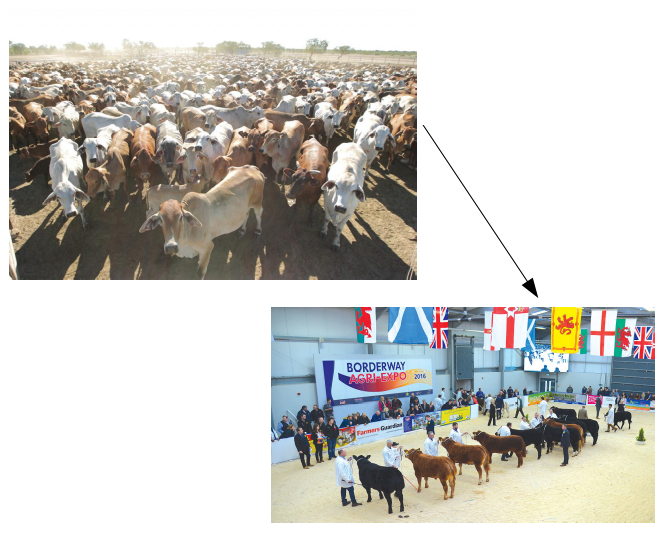
\includegraphics{odg/bestanimal.png}

\note{
\noindent\textbf{Notes}:
\begin{itemize}
\item 
\end{itemize}
}

\end{frame}

\begin{frame}{Phenotypes and Genotypes}
\protect\hypertarget{phenotypes-and-genotypes}{}

\[
P = G + E
\]

where \(P\) and \(E\) are observed and \(G\) is unknown

\note{
\noindent\textbf{Notes}:
\begin{itemize}
\item 
\end{itemize}
}

\end{frame}

\begin{frame}{Improving Animal Populations}
\protect\hypertarget{improving-animal-populations}{}

\begin{itemize}
\tightlist
\item
  Improvement via breeding \(\rightarrow\) long-term
\item
  Two tools
\end{itemize}

\begin{enumerate}
\tightlist
\item
  selection

  \begin{itemize}
  \tightlist
  \item
    process to determine parents of next generation
  \item
    natural selection in wildlife and livestock
  \item
    artificial selection in livestock: fix a goal and rank
  \end{itemize}
\item
  mating

  \begin{itemize}
  \tightlist
  \item
    which animal is bred to which
  \item
    extreme
  \item
    complementary
  \item
    heterosis - crossbreeding
  \end{itemize}
\end{enumerate}

\note{
\noindent\textbf{Notes}:
\begin{itemize}
\item 
\end{itemize}
}

\end{frame}

\begin{frame}{Statistics}
\protect\hypertarget{statistics}{}

\begin{itemize}
\tightlist
\item
  BLUP
\item
  Bayesian methods
\end{itemize}

\note{
\noindent\textbf{Notes}:
\begin{itemize}
\item 
\end{itemize}
}

\end{frame}

\begin{frame}{Computer Science}
\protect\hypertarget{computer-science}{}

\begin{itemize}
\tightlist
\item
  Methods have been developed in 1940's - 1950's
\item
  Progress occured later
\item
  Development of cheap computing power
\end{itemize}

\note{
\noindent\textbf{Notes}:
\begin{itemize}
\item 
\end{itemize}
}

\end{frame}

\begin{frame}{Milk Yield}
\protect\hypertarget{milk-yield}{}

\begin{figure}
\centering
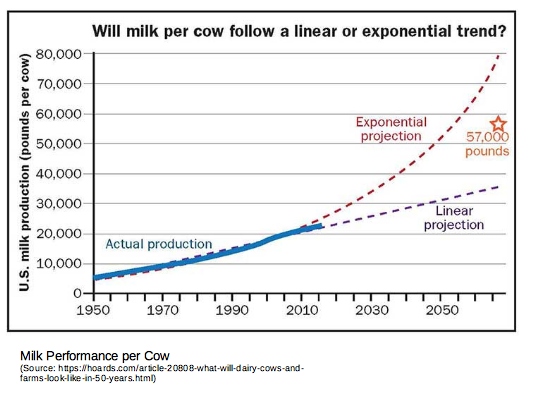
\includegraphics{odg/milkcompperf.png}
\caption{Yearly Milk Yield per Cow in the USA}
\end{figure}

\note{
\noindent\textbf{Notes}:
\begin{itemize}
\item 
\end{itemize}
}

\end{frame}

\begin{frame}{Computer Performance}
\protect\hypertarget{computer-performance}{}

\begin{figure}
\centering
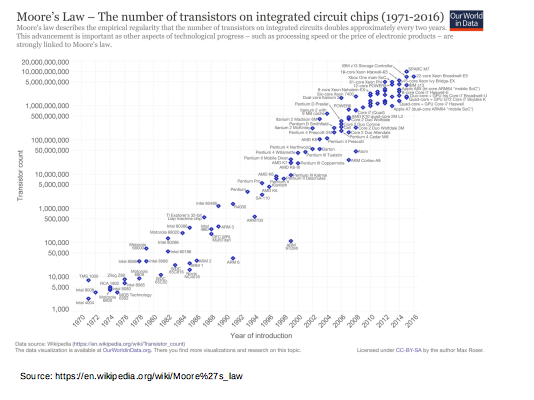
\includegraphics{odg/moorelaw.png}
\caption{Computing Performance According To Moore's Law}
\end{figure}

\note{
\noindent\textbf{Notes}:
\begin{itemize}
\item 
\end{itemize}
}

\end{frame}

\end{document}
